\section{Техническое задание}
\subsection{Основание для разработки}

Основанием для разработки является задание по курсовой работе 
<<Разработка программной библиотеки для шифрования данных по стандарту AES-128>>. 

\subsection{Цель и назначение разработки}

Целью курсовой работы является разработка программной библиотеки для шифрования данных по стандарту AES-128.  

Разработка библиотеки направлена на получение практических навыков проектирования и реализации  алгоритмов, а также на формирование базиса для последующего применения в системах защиты информации.  

Основными задачами данной разработки являются:
\begin{itemize}
	\item реализация функций шифрования данных по стандарту AES-128;
	 \item разработка модуля для формирования ключа;
	\item организация интерфейса для использования библиотеки;
	\item проведение тестирования на примерах входных данных.
\end{itemize}

\subsection{Функции библиотеки}

Библиотека должна включать в себя следующие функции:
\begin{itemize}
	\item основную функцию для шифрования блока данных по алгоритму AES-128;
	\item функцию для задания исходного ключа;
	\item вспомогательные функции для подготовки и преобразования данных;
	\item функцию для приёма входных данных из потока и их передачи на шифрование;
\end{itemize}


Композиция шаблона сайта представлена на рисунке ~\ref{templ:image}.

\begin{figure}[ht]
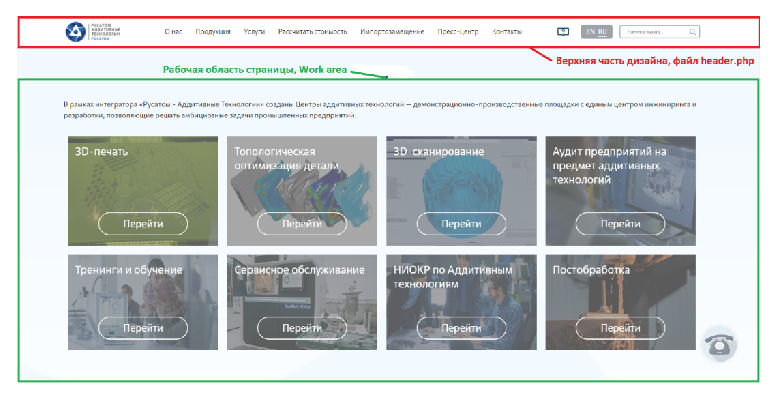
\includegraphics[width=1\linewidth]{templ}
\caption{Композиция шаблона сайта}
\label{templ:image}
\end{figure}
%\vspace{-\figureaboveskip} % двойной отступ не нужен (можно использовать, если раздел заканчивается картинкой)

\subsection{Программный интерфейс}

Для разрабатываемого сайта была реализована модель, которая обеспечивает наглядное представление вариантов использования сайта.

Она помогает в физической разработке и детальном анализе взаимосвязей объектов. При построении диаграммы вариантов использования применяется унифицированный язык визуального моделирования UML.

Диаграмма вариантов описывает функциональное назначение разрабатываемой системы. То есть это то, что система будет непосредственно делать в процессе своего функционирования. Она является исходным концептуальным представлением системы в процессе ее проектирования и разработки. Проектируемая система представляется в виде ряда прецедентов, предоставляемых системой актерам или сущностям, которые взаимодействуют с системой. Актером или действующим лицом является сущность, взаимодействующая с системой извне (например, человек, техническое устройство). Прецедент служит для описания набора действий, которые система предоставляет актеру.

На основании анализа предметной области в программе должны быть реализованы следующие прецеденты:
\begin{enumerate}
\item Просмотр информации о компании.
\item Просмотр информации о продукции компании.
\item Просмотр информации об услугах компании, много услуг, длинный список, не поместится никак в одну строку.
\item Поиск по сайту.
\end{enumerate}

\subsection{Требования к оформлению документации}

Разработка программной документации и программного изделия должна производиться согласно ГОСТ 19.102-77 и ГОСТ 34.601-90. Единая система программной документации.
